\documentclass[]{scrartcl}
\title{Vorlesung Analysis II}
\usepackage{amsmath,amssymb,amsfonts}
\usepackage{stmaryrd}
\usepackage{mathtools}
\usepackage{latexsym}
\usepackage{graphicx}
\usepackage{tikz}
\usepackage{xcolor}
\usepackage{soul}
\usepackage{hyperref}
\usepackage{tipa}
\usepackage[dvipsnames]{xcolor}
\hypersetup{
	colorlinks=true,
	linkcolor=blue,
	filecolor=magenta,      
	urlcolor=cyan,
	pdftitle={Overleaf Example},
	pdfpagemode=FullScreen,
}
\newcommand{\redcircle}[1]{%
	\tikz[baseline=(char.base)]{
		\node[shape=circle, draw=red, text=red, thick, inner sep=1pt] (char) 
		{\textbf{#1}};
	}%
}
\setul{1pt}{1.5pt} % Linienhöhe und Abstand zum Text (optional anpassbar)

\setlength{\topmargin}{-.5in} \setlength{\textheight}{9.25in}
\setlength{\oddsidemargin}{0in} \setlength{\textwidth}{6.8in}
\setlength{\parindent}{0pt}

\begin{document}
	\maketitle
	\textbf{\underline{Teil 1: Differentialgleichung im $\mathbb{R}^n$}}\\
	\\
	\textbf{\underline{an4: Mehrdimensionales Ableiten}}\\
	\\
	\textbf{\underline{\underline{Stichworte:} Richtungsableitung, partielle Ableitung, totale Ableitung, Klein-o}}\\
	\\
	\textbf{\underline{Literatur:}} \setulcolor{blue}\ul{[Hoff], Kapitel 9.4}\\
	\\
	\textbf{4.1. \underline{Einleitung:}} Wir führen den 
	Differenzierbarkeitsbegriff  für Funktionen 
	$\mathbb{R}^n\rightarrow\mathbb{R}^m$ ein: über Richtungsableitungen 
	entlang 
	der Koordinatenachsen gelangen wir zu partiellen Ableitungen. Wir 
	definieren die totale Ableitung und sehen, wie diese mit den partiellen 
	Ableitungen der Komponentenfunktionen berechnet werden kann. Die 
	"Linearsierung" von f ergibt also die Matrix $Df(a)\in\mathbb{R}^{m x n}$ 
	so, dass $f(x) \approx f(a)+Df(a)\cdot(x-a)$ in gute Näherung ist.\\
	\\
	\textbf{4.2 \underline{Konvention:}} Betrachte Funktionen $f:U\rightarrow\mathbb{R}^m$ mit $U \subseteq \mathbb{R}^n$.\\
	Sei $a \in U$ ein \setulcolor{red}\ul{innerer Punkt} von U, d.h. $\exists S 
	> 0: U_a^s\subseteq U.$\\
	Man könnte D füt die Definitionsmenge von f schreiben, tun dies aber wegen Verwechslungsgefahr mit den anderen D's in diesen Kapitel nicht.\\
	\\
	\textbf{4.3.} Hatten: im Fall \underline{n=m=1} ist $f'(a)=\lim_{x\rightarrow a}\frac{f(x)-f(a)}{x-a}$ die Ableitung.  ($\mathbb{R}\supseteq U \ni x \rightarrow a$)\\
	\\
	\textbf{4.4.} \underline{Falls $n>1$}, ist x-a ein Vektor und der Differentialquotient nicht bildbar.\\
	\\
	\textbf{4.5.} \underline{Falls n=1, $m\geq 1$}, ist $\frac{1}{x-a} \cdot 
	(f(x)-f(a))$ der (m-dimensionale) Differenzenquotient \underline{$\in 
	\mathbb{R}^m$},\\
	und \setulcolor{yellow} \ul{Df(a)}:=\setulcolor{red}\ul{$\lim_{x\rightarrow a}\frac{f(x)-f(a)}{x-a}$ die Ableitung}. $(\mathbb{R}\supseteq U \ni x \rightarrow a)$\\
	\begin{figure}[h]
		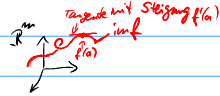
\includegraphics[width=7 cm,height=3cm]{bsp kap 4.5}
	\end{figure}\\
	Sind $f_1,...,f_m$ die Komponentenfunktionen von f, d.h. $f(x)=\begin{pmatrix}
		f_1(x)\\ \vdots \\f_m
	\end{pmatrix}$ für alle x $\in$\underline{$U\subseteq\mathbb{R}$},\\
	also die $f_i:U\rightarrow\mathbb{R}, f_i:=pr_i \circ f$, so ist\\
	\begin{equation}
		\frac{1}{x-a}\cdot(f(x)-f(a))=\frac{1}{x-a}\cdot\begin{pmatrix}
			f_1(x)-f_1(a)\\ \vdots \\ f_m(x)-f_m(a)
		\end{pmatrix}=\begin{pmatrix}
		(f_1(x)-f_1(a))/(x-a)\\ \vdots \\ (f_m(x)-f_m(a))/(x-a)
	\end{pmatrix} \xrightarrow{x\rightarrow a}\begin{pmatrix}
		f_1'(a)\\ \vdots \\ f_m'(a)
		\end{pmatrix},
	\end{equation}\\
	falls alle Komponentenfunktionen $f_i$ diffbar in a sind.\\
	Wir erhalten $Df(a)=\begin{pmatrix}
		f_1'(a)\\ \vdots \\f_m'(a)
	\end{pmatrix} \in \mathbb{R}^m$ in diesem Fall und schreiben auch \setulcolor{yellow} \ul{f'(a)} für Df(a).\\
	\\
	\textbf{4.6 \underline{Bsp.:}} Betrachten $f:\mathbb{R}\rightarrow\mathbb{R}^2, f(x):=\begin{pmatrix}
		x\\x^2
	\end{pmatrix}.$ also :$f_1(x)=x, f_2(x)=x^2, f_1'(x)=1, f_2(x)=2x$, wir erhalten f'(a)=$\begin{pmatrix}
		f_1'(a)\\f_2'(a)
	\end{pmatrix}=\begin{pmatrix}
	1\\2a
	\end{pmatrix}$ für $a\in \mathbb{R}$.\\
	\\
	\textbf{4.7 \underline{Fall n $>$1:}} Mit $a \in U\subseteq \mathbb{R}^n$ und der Konvention, dass a ein innerer Punkt von U ist, können wir und mit $x \in U$ aus verschiedenen Richtungen an a annähern, Ist etwa $v\in \mathbb{R}^n\backslash\{0\}$ ein Vektor, der uns die "Richtung" der Ableitung angeben soll, so wollen wir f "in diese Richtung" ableiten, d.h. die Funktion \setulcolor{yellow} \ul{$f_v$:}$\begin{cases}
		]-s,s[\rightarrow \mathbb{R}^m\\
		t\rightarrowtail f(a+tv)
	\end{cases}$\\ 
	in $(t_0=)0$ ableiten, und haben die Fragestellung auf \setulcolor{blue}\ul{4.5} zurückgeführt. Dabei ist s\textgreater0 geeignet so, dass $U_a^{s||v||}\subseteq U$ ist (damit auch a$\pm s v \in U$ ist). Hier ist es üblich, den Richtungsvektor auf 1 zu \underline{normieren}, d.h. $||v||=1$ vorauszusetzen, damit wir in der Bedingung an s einfach $U_a^s \subseteq U$ schreiben können.\\
	\\
	\textbf{4.8 \underline{Def.:}} Das Ergebnis \setulcolor{yellow}\ul{$D_v f(a)$}:=$\lim_{t\rightarrow 0}\frac{1}{t}\cdot(f(a+tv)-f(a))\in\mathbb{R}^m$, d.h. \setulcolor{red}\ul{$D_v f(a):=f_v'(0)$}, heißt \ul{Richtungsableitung von f in a in Richtung v}.\\
	Diese beschreibt also das Wachstum von f entlang der Geraden $g:\mathbb{R}\rightarrow \mathbb{R}^n$ \\
	g(t):=a+tv (in Parameterform mit $t \in \mathbb{R}$ als Parameter).\\
	\\
	\textbf{4.9 \underline{Bsp.:}}$\bullet f: \mathbb{R}^2 \rightarrow\mathbb{R}^3, \begin{pmatrix}
		x\\y
	\end{pmatrix}\rightarrowtail \begin{pmatrix}
	x+y\\x-y\\2x^2
	\end{pmatrix}$ soll in $a=\begin{pmatrix}
	-3\\4
	\end{pmatrix}$ abgeleitet werden, und zwar \underline{entlang} $v=\begin{pmatrix}
	1\\1
	\end{pmatrix}$ (es sei $||\cdot||=||\cdot||_\infty$).\\
	dazu bilden wir $f_v: t\rightarrowtail f(a+tv)= f \begin{pmatrix}
		-3+t\\4+t
	\end{pmatrix}=\begin{pmatrix}
	1+2t\\-7\\2(-3+t)^2
	\end{pmatrix}=\begin{pmatrix}
	f_{v,1}(t)\\f_{v,2}(t)\\f_{v,3}(t)
	\end{pmatrix}, 
	\begin{cases}
	f_{v,1}(t)=2\\f_{v,2}(t)=0\\f_{v,3}(t)=4(-3+t)
	\end{cases}$\\
	deren Ableitung ist\\
	$D_{\begin{pmatrix}
		1\\1
	\end{pmatrix}} f\begin{pmatrix}
	-3\\4
	\end{pmatrix}'(0)=\begin{pmatrix}
	2\\0\\4\cdot(-3+0)
	\end{pmatrix}=\begin{pmatrix}
	2\\0\\-7
	\end{pmatrix}$.\\
	$\bullet$ Dasselbe f soll entlang der Koordinatenachsen $v_1=\begin{pmatrix}
		\textcolor{red}{1}\\\textcolor{red}{0}
	\end{pmatrix}=: e_1$ und $v_2 =\begin{pmatrix}
		\textcolor{cyan}{0}\\\textcolor{cyan}{1}
	\end{pmatrix}=:e_2$ in $ a= \begin{pmatrix}
		-3\\4
	\end{pmatrix}$ abgeleitet werden. haben $f_{e_1}:t \rightarrowtail f(a+t e_1)=f\begin{pmatrix}
		-3+t\cdot\textcolor{red}{1}\\4+t\cdot\textcolor{red}{0}
	\end{pmatrix}=\begin{pmatrix}
		1+t\\-7+t\\2(-3+t)^2
	\end{pmatrix}\leadsto\begin{cases}
	f_{e_1,1}(t)=1\\f_{e_2,2}(t)=1\\f_{e_3,3}(t)=4(-3+t)
	\end{cases}$\\
	mit Abl. \underline{\underline{$D_{e_1}f\begin{cases}
				-3\\4
			\end{cases}$}}=$f_{\begin{pmatrix}
		1\\0
	\end{pmatrix}}'(0)=\begin{pmatrix}
	1\\1\\-12
	\end{pmatrix},$\\
	und mit $f_{e_2}: t\rightarrowtail f(a+t e_2)=f\begin{pmatrix}
		-3t\cdot\textcolor{cyan}{0}\\4+t\cdot\textcolor{cyan}{1}
	\end{pmatrix}=\begin{pmatrix}
		1+t\\-7-t\\18
	\end{pmatrix}\leadsto\begin{cases}
	f_{e_2,1}(t)=1\\f_{e_2,2}(t)=1\\f_{e_2,3}(t)=4(-3+t)
	\end{cases}$\\SCHAU NACH WAS HIER RICHTIG IST E 2 ODER E 1-3!!!!!!!!!!\\
	mit Ableitung \underline{\underline{$D_{e_1}f\begin{pmatrix}
			-3\\4
		\end{pmatrix}$}}=$f_{\begin{pmatrix}
		0\\1
		\end{pmatrix}}'(0)=\begin{pmatrix}
	1\\-1\\0
	\end{pmatrix}$.\\
	\\
	\textbf{4.10 \underline{Def.:}} Für $j\in\{1,...,n\}$ heißt die Richtungsableitung \setulcolor{yellow} \ul{$D_jf(a)=\frac{\delta f}{\delta x_j}$}:=\setulcolor{red}\ul{$D_{e_j}f(a)$} $\in \mathbb{R}^m$\\
	von f in a in Richtung des j-ten Kanonischen Einheitsvektors $e_j = (0,...,0,\textcolor{cyan}{1}(\text{setlle j}),0,...,0)\in\mathbb{R}^n\\$
	(d.h. in richtung der j-ten Koordinatenachse)\\
	dir \setulcolor{red}\ul{j-te partielle ableitung von f in a}.\\
	\\
	\textbf{4.11 \underline{Bem.:}}$\bullet$ Für m=1 erhält man dies Ableitung $\in \mathbb{R}$ durch Ableiten nach der j-ten Variable, denn 
	\begin{align}
		D_{\textcolor{cyan}{e_j}}f(a)&= \lim\limits_{t\rightarrow 0}\frac{1}{t}(f(a+t\textcolor{cyan}{e_j})-f(a))\\
		&=\lim\limits_{t\rightarrow0}\frac{1}{t}\cdot(f(...,a_{j-1},a_j+t\cdot\textcolor{cyan}{1}, a_{j+1},...)-f(...,a_{j-1},a_j,a_{j+1},...)),
	\end{align} \\
	\\
	\textbf{4.12 \underline{Bsp.:}} $ f:\mathbb{R}^3\rightarrow\mathbb{R}, 
	f\begin{pmatrix}
		x\\y\\z
	\end{pmatrix} = 2x+y^3-z^2.$ Sei $j\in \{1,2,3\}, a=\begin{pmatrix}
	u\\v\\w
\end{pmatrix} \in \mathbb{R}.$\\
Dann ist \begin{align}
	D_{\textcolor{cyan}{e_2}} f(a)&= \lim\limits_{t\rightarrow 
	0}\frac{1}{t}(f\begin{pmatrix}
		u\\v+t\cdot\textcolor{cyan}{1}\\w
	\end{pmatrix}-f\begin{pmatrix}
	u\\v\\w
\end{pmatrix}).\\
&=\lim\limits_{t\rightarrow0}\frac{1}{t}\cdot(2u+(v+t)^3-w^2-(2u+v^3-w^2))\\
&=\lim\limits_{t\rightarrow 
0}\frac{1}{t}\cdot(t^3+3vt^2+3v^2t)=\underline{3v^2}\frac{\delta f}{\delta 
y}(\begin{pmatrix}
	u\\v\\w
\end{pmatrix}),
\end{align}\\
entsprechend $D_{e_1}f(\begin{pmatrix}
	x\\y\\z
\end{pmatrix})=$\underline{2}, $D_{e_2}f\begin{pmatrix}
	x\\y\\z
\end{pmatrix}=\frac{\delta f}{\delta z}(\begin{pmatrix}
	u\\v\\w
\end{pmatrix})=$\underline{-2w}.\\
\\
\textbf{4.13. \underline{Bem.:}} Ist $f: U\rightarrow \mathbb{R}^m$ mit 
$U\subseteq \mathbb{R}^n$, so erhält man die j-te partille Ableitung 
$\frac{\delta f}{\delta x_j}$ durch Bilden der j-ten partiellen Ableitung der 
Komponentenfunktion $f_1,...,f_m,$ nähmlich: ist $f=\begin{pmatrix}
	f_1\\\vdots\\f_m
\end{pmatrix}$ mit $f_i : U\rightarrow\mathbb{R}, f_i=pr_i \circ f,$\\
so ist $D_{e_j} f(a)=\lim\limits_{t\rightarrow 
0}\frac{1}{t}\cdot(\begin{pmatrix}
	f_1\\\vdots\\f_m
\end{pmatrix}(a+t\textcolor{cyan}{e_j})-\begin{pmatrix}
	f_1\\\vdots\\f_m
\end{pmatrix}(a))=\lim\limits_{t\rightarrow0}\frac{1}{t}\cdot\begin{pmatrix}
	f_1(a+t\cdot\textcolor{cyan}{e_j})-f_1(a)\\\vdots\\f_m(a+t\cdot\textcolor{cyan}{e_j})-f_m(a)
\end{pmatrix}$\\
=$\begin{pmatrix}
	D_{e_j}f_1(a)\\D_{e_j}f_2(a)\\\vdots\\D_{e_j}f_m(a)
\end{pmatrix}$, bzw. $\frac{\delta f}{\delta x_j}=\begin{pmatrix}
	\frac{\delta f_1}{\delta x_j}\\\vdots\\\frac{\delta f_m}{\delta x_j}
\end{pmatrix}$, \underline{jede} Komponente $f_j$ wird nach der j-ten Variablen 
abgeleitet!\\
\\
\textbf{4.14. \underline{Bsp.:}} nochmal \setulcolor{blue} \ul{4.9.}, d.h. 
$f:\mathbb{R}^2\rightarrow\mathbb{R}^3, \begin{pmatrix}
	x\\y
\end{pmatrix}\rightarrowtail\begin{pmatrix}
	x+y\\x+y\\2x^2
\end{pmatrix}.$\\
Es sollen die partiellen Ableitung berechnet werden. Laut \ul{4.13.} ist 
(einfacher als in \ul{4.9.}): $D_1f\begin{pmatrix}
	x\\y
\end{pmatrix}=\frac{\delta  f}{\delta x}\begin{pmatrix}
	x\\y
\end{pmatrix}=\begin{pmatrix}
	1\\1\\4x
\end{pmatrix}, D_2f\begin{pmatrix}
	x\\y
\end{pmatrix}=\frac{\delta f}{\delta y}\begin{pmatrix}
	x\\y
\end{pmatrix}=\begin{pmatrix}
	1\\-1\\0
\end{pmatrix},$\\
also $D_1f\begin{pmatrix}
	-3\\4
\end{pmatrix}=\begin{pmatrix}
	1\\1\\4\cdot(-3)
\end{pmatrix}=\begin{pmatrix}
	1\\1\\12
\end{pmatrix}, D_2f\begin{pmatrix}
	-3\\4
\end{pmatrix}=\begin{pmatrix}
	1\\-1\\0
\end{pmatrix}.$\\
\\
\textbf{4.15. \underline{Beobachtung:}} Kennt man alle partillen Ableitung, ist 
auf Anhieb nicht klar, ib die Funktion f "mehrdimensional§ differenzierbar ist, 
denn f kann partiell diffbar in Richtung aller $e_1,...,e_n$ in a sein, aber 
so, dass f noch nicht einmal stetig in a ist:\\
\\
\textbf{4.16. \underline{Bsp.:}} $f:\mathbb{R}^2\rightarrow\mathbb{R}, 
f\begin{pmatrix}
	x\\y
\end{pmatrix}=\begin{cases}
	\frac{xy}{x^2+y^2}&, \text{ falls } \begin{pmatrix}
		x\\y
	\end{pmatrix}\neq\begin{pmatrix}
	0\\0
\end{pmatrix},\\
0 &, \text{ falls } x=y=0, a=\begin{pmatrix}
	0\\0
\end{pmatrix}.
\end{cases}$\\
Die beiden partiellen Ableitungen sind $D_1f\begin{pmatrix}
	0\\0
\end{pmatrix}=\lim\limits_{t\rightarrow0}\frac{1}{t}(f\begin{pmatrix}
	t\\0
\end{pmatrix}-f\underbrace{\begin{pmatrix}
	0\\0
\end{pmatrix}}_{=0})=\lim\limits_{t\rightarrow 0}\frac{1}{t}\cdot0=0$ und 
$D_2f\begin{pmatrix}
	0\\0
\end{pmatrix}= \lim\limits_{t\rightarrow0}\frac{1}{t}(f\begin{pmatrix}
	0\\t
\end{pmatrix}-f\underbrace{\begin{pmatrix}
	0\\0
\end{pmatrix}}_{=0})=\lim\limits_{t\rightarrow 0}\frac{1}{t}\cdot0=0,$\\
aber $\lim\limits_{\begin{pmatrix}
	x\\y
\end{pmatrix}\rightarrow\begin{pmatrix}
	0\\0
\end{pmatrix}}f\begin{pmatrix}
	x\\y
\end{pmatrix}$ existiert nicht,\\
weil $f\begin{pmatrix}
	x\\0
\end{pmatrix}\xrightarrow{x\rightarrow0}0$, aber $ f\begin{pmatrix}
	x\\x
\end{pmatrix}=\frac{1}{2}\xrightarrow{x\rightarrow0}\frac{1}{2}\neq0.$ Hier ist 
y=x gewählt, bzw die Richtung $v=\begin{pmatrix}
	1\\1
\end{pmatrix}!$\\
an verschiedenen Richtungen können verschiedene Funktionsgrenzwerte 
herauskommen, d.h. f ist unstetig in $a=\begin{pmatrix}
	0\\0
\end{pmatrix}$,  s. auch Bsp. \ul{3.22}.\\
\\
\textbf{4.17. \underline{Motivation:}} Das richtige Konzept zum 
mehrdimensionalen Ableiten ist die totale Ableitung und ist die 
verallgemeinerung von \ul{An 11.4.3},\\
\underline{Erinnerung:}\\
$f:U\rightarrow\mathbb{R}$ diff'bar in $a\in U\subseteq\mathbb{R}, U$ ein 
offenes Intervall\\
$\Leftrightarrow \exists A\in\mathbb{R} \exists r:U\rightarrow \mathbb{R}$ 
stetig, $r(a)= 0: f(x)=f(a)+A\cdot(x-a)+r(x)\cdot(x-a),$\\
mit der Interpretation: $f(x)-f(a)-A(x-a)=r(x)\cdot(x-a)$\\
geht schneller gegen 0 als $|x-a|$.\\
Auch der \ul{Satz von  Taylor An 19.3} macht diese Aussage; nur wird dort 
"$r(x)\cdot(x-a)$" noch näher spezifiziert, was die Aussage der Diff'barkeit 
verfeinert.\\
\\
Für eine Funktion, die "schneller gegen 0 geht als $|x-a|$", wird eine 
mehrdimensionale Definition wie folgt gegeben:\\
\textbf{4.18. \underline{Def.:}} Für $\varphi:U\rightarrow\mathbb{R}^m, x\in U$ 
mit $\exists\epsilon\textgreater0:U_a^\epsilon\subseteq U\subseteq\mathbb{R}^n$ 
sei\\
\setulcolor{yellow}\ul{$\varphi=\sigma(||x-a||)$}:$\Leftrightarrow 
\frac{1}{||x-a||}$\setulcolor{red}\ul{$\varphi(x)\xrightarrow{x\rightarrow 
a}0$}.\\
Sprich: $\varphi(x)$ ist "\underline{klein o}" von $||x-a||$.\\
Diese Klein-o-Aussage ist eine Eigenschaft von $\varphi$.\\
Wenn das Symbol $o(||x-a||)$ in einer Formel vorkommt, steht dieses dort 
stellvertretend für eine Funktion, die diese "Klein-o"-Eigenschaft hat.\\
\\
Somit geben wir die allgemeinste Def. für \underline{mehrdimensionale 
Diff'barkeit} (für $\mathbb{R}^n\supseteq U \xrightarrow{f}\mathbb{R}^m$):\\
\textbf{4.19. \underline{Def.:}} Geg. sei $f:U\rightarrow\mathbb{R}^m$ mit 
$\exists \epsilon\textgreater0: U_a^\epsilon\subseteq U.\\
\bullet$ Dann heißt \setulcolor{red}\ul{f in a diff'bar}: $\Leftrightarrow 
\exists A \in \mathbb{R}^{m x n}$:\\
$f(x)=f(a)+A\cdot(x-a)+o(||x-a||)$ auf U.\\
$\bullet$ Ist f in a diff'bar, dann heißt \setulcolor{yellow}\ul{$f'(a)=Df(a)$} 
$:=A\in\mathbb{R}^{m x n}$\\
die \setulcolor{red}\ul{erste Ableitung} bzw. \ul{totale Ableitung} von f in 
a.\\
\\
\textbf{4.20. \underline{Bem.:}} Dabei ist A eindimensional bestimmt (laut 
\setulcolor{blue}\ul{Bem. 4.26} unten).\\
\\
Beispiele: Hier sei stets $a\in U, \exists\epsilon 
\textgreater0:U_a^\epsilon\subseteq U\subseteq\mathbb{R}^n.$\\
\textbf{4.21. \underline{Bsp.:}} f sei die \setulcolor{green}\ul{Konstante 
Abb.} $f:U\rightarrow\mathbb{R}^m, x\rightarrowtail c$ mit $c\in\mathbb{R}^m$ 
fest.\\
Dann ist f in $a\in U$ diff'bar und \ul{$f'(a)=\mathcal{O}$}$\in\mathbb{R}^{m x 
n}$ (die m x n-Nullmatrix!).\\
\underline{Bew.:} $f(x)=c=c+o\cdot(x-a)+o \leftarrow \in\mathbb{R}^m$ 
Nullvektor.\\
\strut\hfill$\square$\\
\textbf{4.22. \underline{Bsp.:}} $f\in Hom(\mathbb{R}^n,\mathbb{R}^m),$ d.h. 
$f:\mathbb{R}^n
\rightarrow\mathbb{R}^m$ linear und \ul{$f(x)=Mx$} für $M\in\mathbb{R}^{m x 
n}$.\\
Dann ist f in $a\in\mathbb{R}^n$ diff'bar und \ul{f'(a)=M} $\in\mathbb{R}^{m x 
n}$.\\
\underline{Bew.:} $f(x) = Mx =M(x-a+a)=\underbrace{Ma}_{f(a)}+M(x-a)+o.$\\
\strut\hfill$\square$\\
\underline{Spezielles Bsp.:} $f:\mathbb{R}^2\rightarrow\mathbb{R}, 
M:=(1,1)\in\mathbb{R}^{1x2}$, \ul{f(x)=Mx}=(1,1)$\begin{pmatrix}
	\xi_1\\\xi_2
\end{pmatrix}=\xi_1+\xi_2$\\
ist diff'bar in $a\in\mathbb{R}^2$ und \ul{$f'(a)=(1,1)$} $\in 
\mathbb{R}^{1x2}.$\\
\\
\textbf{4.23. \underline{Bsp.:}} $f:\mathbb{R}^2\rightarrow\mathbb{R}$, 
\ul{$f\begin{pmatrix}
	\xi_1\\\xi_2
\end{pmatrix}$}=$\xi_1\xi_2$, ist diff'bar in jedem $a=\begin{pmatrix}
	\alpha_1\\\alpha_2
\end{pmatrix}\in\mathbb{R}^2$,\\
und \ul{$f'\begin{pmatrix}
	\alpha_1\\\alpha_2
\end{pmatrix}=(\alpha_2,\alpha_1)$}$\in\mathbb{R}^{1x2}$.\\
\underline{Bew.:}\\
\begin{align}
	f(x)=\xi_1\xi_2&=(\alpha_1+(\xi_1-\alpha_1))(\alpha_2+(\xi_2-\alpha_2))\\
	&=\alpha_1\alpha_2+(\alpha_2,\alpha_1)\cdot\begin{pmatrix}
		\xi_1-\alpha_1\\\xi_2-\alpha_2
	\end{pmatrix}+(\xi_1-\alpha_1)\cdot(\xi_2-\alpha_2)\\
	&=f(a)+(\alpha_2,\alpha_1)\cdot(x-a)+(\xi_1-\alpha_1)\cdot(\xi_2-\alpha_2)
\end{align}\\
mit $||(\xi_1-\alpha_1)\cdot(\xi_2-\alpha_2)||\leq||\begin{pmatrix}
	\xi_1-\alpha_1\\\xi_2-\alpha_2
\end{pmatrix}||_\infty^2=o(||x-a||),$\\
denn $\frac{1}{||x-a||}\cdot||x-a||^2=||x-a||\xrightarrow{x\rightarrow a}0.$\\
\strut\hfill$\square$\\
\textbf{4.24 \underline{Bsp.:}} $f:\mathbb{R}^n\rightarrow\mathbb{R},$ 
\ul{$f(x)=\textless x,x\textgreater$} ist diff'bar in jedem 
$a\in\mathbb{R}^n$,\\
under \ul{$f'(a)=\textless 2a,\cdot\textgreater=2a^T$}$\in\mathbb{R}^{1xn}.$\\
\underline{Bew.:}
\begin{align}
	f(x)&=\textless x,x\textgreater=\textless a+(x-a), a+(x-a)\textgreater\\
	&=\textless a,a\textgreater+2\textless a,x-a\textgreater+\textless 
	x-a,x-a\textgreater\\
	&=f(a)+2a^T\cdot(x-a)+\underbrace{||x-a||_2^2}_{=o(||x-a||).}
\end{align}\\
\strut\hfill$\square$\\
Erste Eigenschaft des eindimensionalen Differenzierens übertragen sich:\\
\textbf{4.25. \underline{Bem.:}} \ul{f in a diff'bar} $\Rightarrow$ \ul{f in a 
stetig}.\\
\underline{Bew.:}
\begin{equation}
	||f(x)-f(a)||_\infty\leq \underbrace{||A(x-a)||_\infty}_{\leq n 
	\max_{i,j}|\alpha_{ij}|\cdot||x-a||_\infty\xrightarrow{x\rightarrow 
	0}0}+\underbrace{||o(||x-a||)||_\infty}_{\xrightarrow[x\rightarrow a]{ 
	}0}\xrightarrow{x\rightarrow a}0.
\end{equation}\\
\strut\hfill$\square$\\
\textbf{4.26. \underline{Bem.:}} f \ul{in a diffbar} $\Leftrightarrow \forall i 
\in \{1,...,m\}:$\ul{$f_i=pr_j\circ f$}:$D\rightarrow\mathbb{R}$ \ul{diff'bar 
in a} und dabei gilt:\\
$f'(a)=\begin{pmatrix}
	f_1'(a)\\\vdots\\f_m'(a)
\end{pmatrix}\in \mathbb{R}^{m x n},$\\
worin\ul{jede Ableitung $f_i'(a)\in\mathbb{R}^{1 x n}$} ein \ul{Zeilenvektor} 
ist. (Somit ist die Matrix f'(a) eindeutig bestimmt).\\
\underline{Bew.:}"$\Rightarrow$": $\forall i \in \{1,...,m\}::$\\
$pr_i \circ f(x)==pr_i(f(x))=pr_i(f(a))+pr_i(f'(a)(x-a))+pr_i(o(||x-a||))\\$
d.h. $f_i(x)= f_i(a)+f_i'(a)\cdot(x-a)+o(||x-a||).$\\
"$\Leftarrow$": $f(x)=\begin{pmatrix}
	f_1(x)\\\vdots\\f_m(x)
\end{pmatrix}=\begin{pmatrix}
f_1(a)+f_1'(a)(x-a)+o(||x-a||)\\\vdots\\f_m(a)+f_m'(a)(x-a)+o(||x-a||)
\end{pmatrix}=f(a)+\begin{pmatrix}
	f_1'(a)\\\vdots\\f_m'(a)
\end{pmatrix}\cdot(x-a)+o(||x-a||).$\\
\strut\hfill$\square$\\



\end{document} 